The first scenario concerns the yearly citations of articles published in 1980 until 2023, where we fit equation (\ref{eq:number_of_attachments_over_time}) to the the yearly citation histogram.

%==================================
% FIGURE
%==================================
\begin{figure}[H]
    \centering\includegraphics[scale=0.35, angle=270]{figs/citations.eps}
    \caption{}
    \label{fig:citations_fit}
\end{figure}

\begin{table}[H]
\begin{tabular}{|c c c c c|}
\hline
\# of Citations & RMS of Residuals & $\sigma$ & $\alpha$ & $M_{0}$    \\ \hline
1666 & 8.7546 & 15.85745 & 0.314334 & 27.8297 \\ \hline
550 & 4.03577 & 17.05420 & 0.316177 & 8.54389 \\ \hline
124 & 1.31794 & 10.50930 & 3.86016 & 5.11926e-05\\ \hline
\end{tabular}
\end{table}

If figure \ref{fig:citations_fit} there are two kinds of citation patterns, one where the number of citations increases rapidly followed by a slow decrease as time goes by. And the second kind, where the number of citations increases slowly but takes on afterwards, followed again by decrease after its peak. Both kinds of adoptions curves are well adjusted by our innovation model

The next set of data corresponds to the mutations for SARS-CoV-2 over time, where we consider the first detect strain as being the one found in Wuhan (hCoV-19/Wuhan/Hu-1/2019). The data was obtained by digitizing Fig. 4 (b) from \cite{Lee2022}, where a similar analysis is applied.
We use the mutations from root (the first found strain) as a measure of time and \textcolor{red}{tenho que ler melhor sobre o tratamento de dados que o Lee faz para obter esse gráfico...}

%==================================
% FIGURE
%==================================
\begin{figure}[H]
    \centering\includegraphics[scale=0.35, angle=270]{figs/cladecount.eps}
    \caption{}
    \label{fig:}
\end{figure}

\begin{table}[H]
\begin{tabular}{|c c c c c|}
\hline
Region & RMS of Residuals & $\sigma$ & $\alpha$ & $M_{0}$ \\ \hline
North America & 0.228755  & 2.745150 & 2.805370  & 0.126760 \\ \hline
Europe        & 0.34383 & 3.385185 & 1.393420  & 1.189050 \\ \hline
\end{tabular}
\end{table}

The third set of data correspond to Google searches of the social platforms known as Facebook and Snapchat, such data is provided openly by the Google Trends platform. We use the searches as a form of diagnosing the popularity of these two social medias that have existed for more than 10 years, the months axis represent the number of months elapsed since the first citation of the terms "Facebook" and "Snapchat" in Google Trends platform.

%==================================
% FIGURE
%==================================
\begin{figure}[H]
    \centering\includegraphics[scale=0.35, angle=270]{figs/google_trends.eps}
    \caption{}
    \label{fig:social_media}
\end{figure}

\begin{table}[H]
\begin{tabular}{|c c c c c|}
\hline
Social Media & RMS of Residuals & $\sigma$ & $\alpha$ & $M_{0}$ \\ \hline
Facebook & 8.55684  & 32.3251 & 5.4501  & 1.23955e-08 \\ \hline
Snapchat & 10.0758 & 20.1910 & 4.8127  & 2.11764e-06 \\ \hline
\end{tabular}
\end{table}

Equation \ref{eq:number_of_attachments_over_time}, agrees for most part of the data, where the adoption of both social medias assumes a power-law and the detachment is Gaussian-like. For Snapchat, approximately at month 100 since the first Google search, the rate of detachment changes, our belief is that this is caused by an external factor, such as the pandemics, as month 100 corresponds approximately to November 2019, where Covid-19 began spreading throughout the world and the countries began restricting the transit of people. The restriction most likely changed the amount of time that people interacted with social media, which may be the leading factor for changing the search dynamics for the term "Snapchat". We believe the same happened for "Facebook", whose detachment starts to deviate from the fitted function approximately at month 180 which coincides with the latter half of 2019.